\documentclass[tikz]{standalone}

\usepackage{transparent}
\usepackage{nicematrix}
\usetikzlibrary{matrix, fit}
\usetikzlibrary{backgrounds}
\usetikzlibrary{positioning}
\usetikzlibrary{decorations.pathreplacing}

\newlength{\mycellheight}
\newlength{\innermargin}
\newlength{\cornerrad}
\newlength{\vsep}
\newlength{\msep}  % Offset from center
\newlength{\hsep}  % Offset between blocks
\newlength{\thirdlevelsep}

\newcommand{\0}{{\transparent{0} \resizebox{\mycellheight}{\mycellheight}{0}}}

\begin{document}
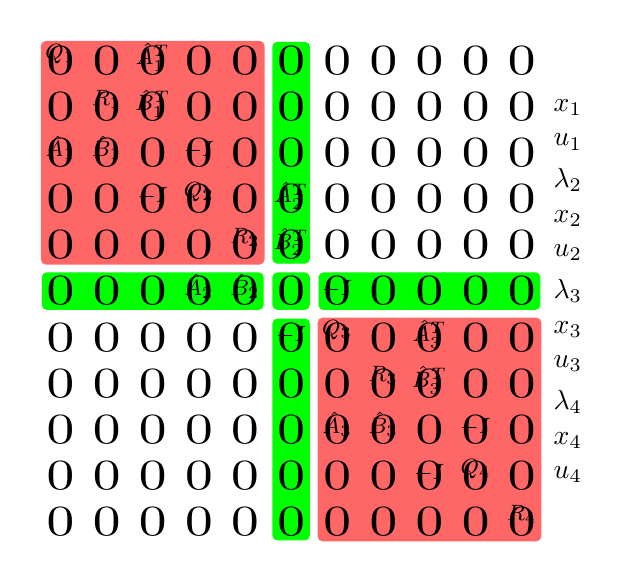
\begin{tikzpicture}
    
    \setlength{\mycellheight}{1.0em}
    \setlength{\innermargin}{-0.2em}
    \setlength{\cornerrad}{1.5pt}
    \setlength{\vsep}{1.2cm}
    \setlength{\msep}{0.7cm}
    \setlength{\hsep}{4.5cm}
    % \setlength{\thirdlevelsep}{\vsep/2}

    {
    \matrix[matrix of math nodes] (m) 
    {
        \0&\0&\0&\0&\0&\0&\0&\0&\0&\0&\0\\
        \0&\0&\0&\0&\0&\0&\0&\0&\0&\0&\0\\
        \0&\0&\0&\0&\0&\0&\0&\0&\0&\0&\0\\
        \0&\0&\0&\0&\0&\0&\0&\0&\0&\0&\0\\
        \0&\0&\0&\0&\0&\0&\0&\0&\0&\0&\0\\
        \0&\0&\0&\0&\0&\0&\0&\0&\0&\0&\0\\
        \0&\0&\0&\0&\0&\0&\0&\0&\0&\0&\0\\
        \0&\0&\0&\0&\0&\0&\0&\0&\0&\0&\0\\
        \0&\0&\0&\0&\0&\0&\0&\0&\0&\0&\0\\
        \0&\0&\0&\0&\0&\0&\0&\0&\0&\0&\0\\
        \0&\0&\0&\0&\0&\0&\0&\0&\0&\0&\0\\
    };
    \matrix[matrix of math nodes] at (10em,0) (x)
    {
        x_1 \\ u_1 \\ \lambda_2 \\ x_2 \\ u_2 \\ \lambda_3 \\ x_3 \\ u_3 \\ \lambda_4 \\ x_4 \\ u_4 \\
    };
    }

    \begin{scope}[on background layer]
        \node[fit=(m-1-6)(m-5-6), draw=green, fill=green, rounded corners=\cornerrad, inner sep=\innermargin] (D) {};
        \node[fit=(m-6-1)(m-6-5), draw=green, fill=green, rounded corners=\cornerrad, inner sep=\innermargin] (Dt) {};
        \node[fit=(m-7-6)(m-11-6), draw=green, fill=green, rounded corners=\cornerrad, inner sep=\innermargin] (E) {};
        \node[fit=(m-6-7)(m-6-11), draw=green, fill=green, rounded corners=\cornerrad, inner sep=\innermargin] (Et) {};
        \node[fit=(m-6-6)(m-6-6), draw=green, fill=green, rounded corners=\cornerrad, inner sep=\innermargin] (B) {};

        \node[fit=(m-1-1)(m-5-5),   draw=red!60!white, fill=red!60!white, very thick, rounded corners=\cornerrad, inner sep=\innermargin] (A) {};
        \node[fit=(m-7-7)(m-11-11), draw=red!60!white, fill=red!60!white, very thick, rounded corners=\cornerrad, inner sep=\innermargin] (C) {};
        % \node[fit=(m-10-6)(m-11-6), draw=red, very thick, rounded corners=\cornerrad, inner sep=0em] {};

    \end{scope}
    \foreach \x/\y/\k in {1/2/1,4/5/2,7/8/3,10/11/4} {
        \node[fit=(m-\x-\x), text height=8pt] {\footnotesize $Q_{\k}$};
        \node[fit=(m-\y-\y), text height=8pt] {\footnotesize $R_{\k}$};
    }
    \node[fit=(m-1-3), text height=10pt] {\footnotesize $\hat{A}_1^T$};
    \node[fit=(m-2-3), text height=10pt] {\footnotesize $\hat{B}_1^T$};
    \node[fit=(m-4-3), text height=10pt] {\footnotesize $-I$};
    \node[fit=(m-4-6), text height=10pt] {\footnotesize $\hat{A}_2^T$};
    \node[fit=(m-5-6), text height=10pt] {\footnotesize $\hat{B}_2^T$};
    \node[fit=(m-7-6), text height=10pt] {\footnotesize $-I$};
    \node[fit=(m-7-9), text height=10pt] {\footnotesize $\hat{A}_3^T$};
    \node[fit=(m-8-9), text height=10pt] {\footnotesize $\hat{B}_3^T$};
    \node[fit=(m-10-9), text height=10pt] {\footnotesize $-I$};

    \node[fit=(m-3-1), text height=10pt] {\footnotesize $\hat{A}_1$};
    \node[fit=(m-3-2), text height=10pt] {\footnotesize $\hat{B}_1$};
    \node[fit=(m-3-4), text height=10pt] {\footnotesize $-I$};
    \node[fit=(m-6-4), text height=10pt] {\footnotesize $\hat{A}_2$};
    \node[fit=(m-6-5), text height=10pt] {\footnotesize $\hat{B}_2$};
    \node[fit=(m-6-7), text height=10pt] {\footnotesize $-I$};
    \node[fit=(m-9-7), text height=10pt] {\footnotesize $\hat{A}_3$};
    \node[fit=(m-9-8), text height=10pt] {\footnotesize $\hat{B}_3$};
    \node[fit=(m-9-10), text height=10pt] {\footnotesize $-I$};
    

    % \node[below] at (A.west) (Alabel) {$A$};
    % \node[above] at (C.east) (Clabel) {$C$};

    % \draw[decorate,decoration={brace,amplitude=4pt, raise=4pt, aspect=0.5}] 
    %     (A.south west) -- (A.north west) 
    %     node[pos=0.5,left,xshift=-1em] {$A$};
    % \draw[decorate,decoration={brace,amplitude=4pt, raise=4pt, aspect=0.5}] 
    %     (C.north east) -- (C.south east) 
    %     node[pos=0.5,right,xshift=+1em] {$C$};
    % \draw[decorate,decoration={brace,amplitude=4pt, raise=4pt, aspect=0.5}] 
    %     (D.north east) -- (D.south east) 
    %     node[pos=0.5,right,xshift=+1em] {$D$};
    % \draw[decorate,decoration={brace,amplitude=4pt, raise=4pt, aspect=0.5}] 
    %     (E.south west) -- (E.north west) 
    %     node[pos=0.5,left,xshift=-1em] {$E$};
\end{tikzpicture}
\end{document}